\documentclass[11pt]{article}
\usepackage{fullpage}
\usepackage{setspace}
\usepackage{amsmath}
\usepackage{fancyvrb}
\usepackage{enumerate}
\usepackage{pgfplots}
\usepackage{graphicx}
\usepackage{float}
\usepackage{multirow}
\usepackage[format=hang,labelsep=quad]{caption}
\usepackage{subfig}
\usepackage{array}
\usepackage{multirow}
%\usepackage{subcaption}

\renewcommand\thesubfigure{\roman{subfigure}}


\begin{document}
\noindent\large{Math 5365}\\
\large{Data Mining 1}\\
\large{Homework 10}\\
\large{Mary Barker}
\doublespace
\begin{enumerate}

\item Split germancredit.csv into 70\% training and 30\% test data. Create models for
      predicting default using the following learning algorithms, and find the area 
      under the ROC curve for each model.

  \begin{enumerate}
     \item Decision tree

     The area under the curve for decision tree is 0.6309. 
     \begin{center}
       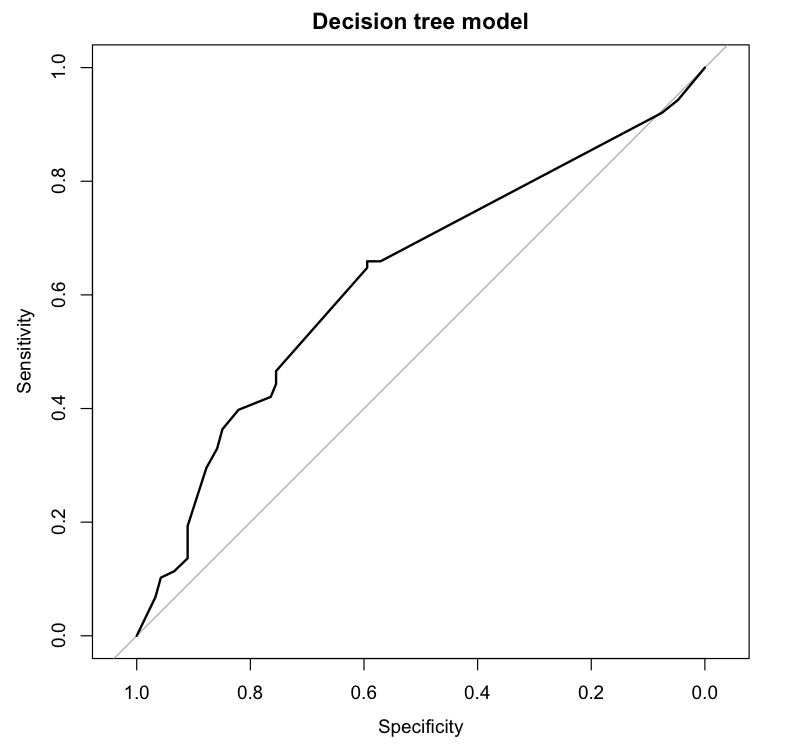
\includegraphics[scale=0.35]{pix/decision_tree}
     \end{center}

     \item Weighted k-nearest neighbors

     The area under the curve for weighted k nearest neighbors with k = 3 is 0.6785
     \begin{center}
       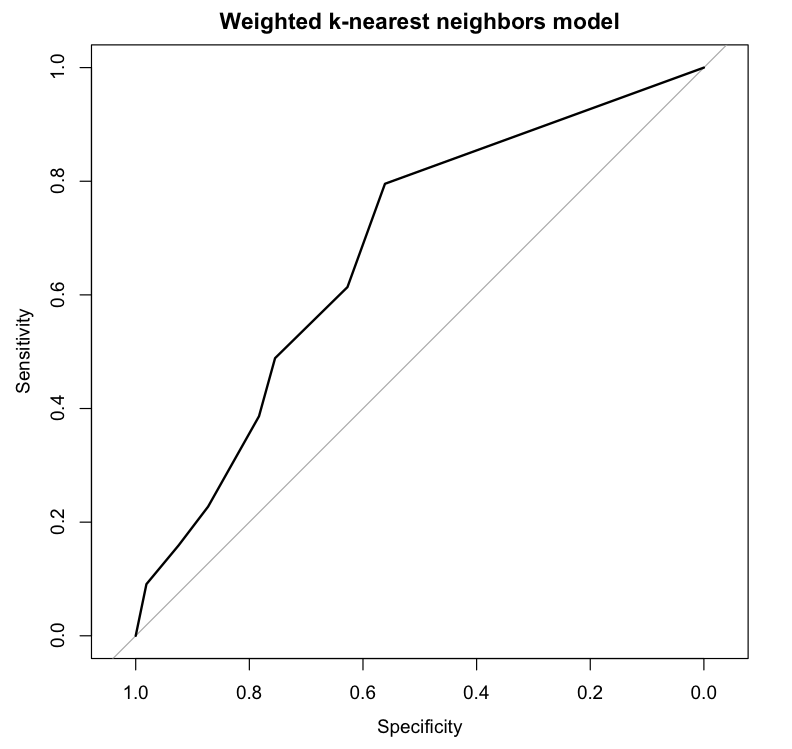
\includegraphics[scale=0.35]{pix/wkknn}
     \end{center}

     \item Naive Bayes

     The area under the curve for Naive Bayes is 0.7535. 
     \begin{center}
       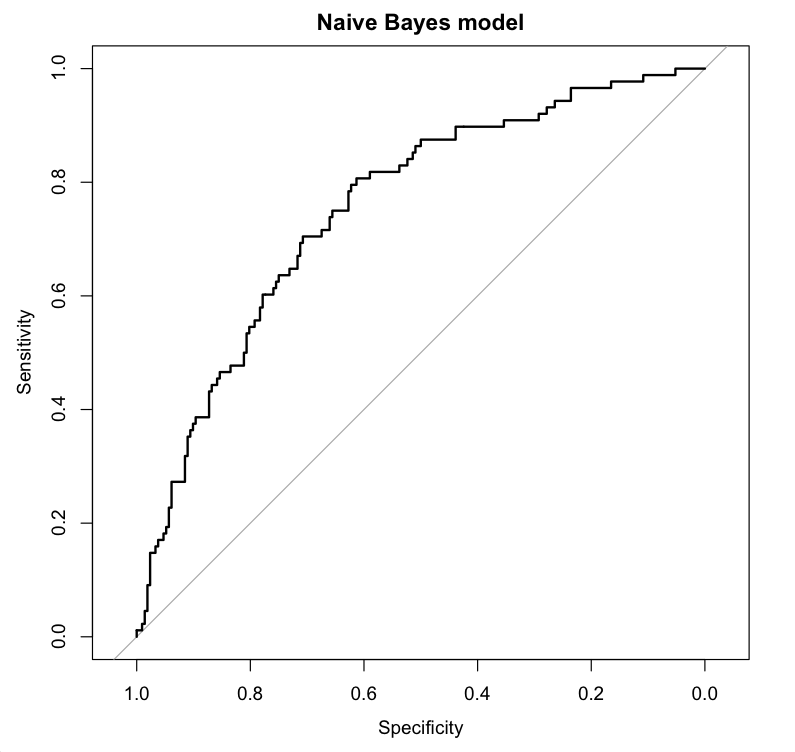
\includegraphics[scale=0.35]{pix/naiveBayes}
     \end{center}

  \end{enumerate}

By visual inspection and an evaluation of the area under each curve, the \verb|naiveBayes| model gives the best 
results.  

\item Consider the following cost structure
  \begin{itemize}
    \item Predicting someone will default when they don`t: \$5,000 in lost interest payments.

    \item Predicting someone will not default when they do: \$20,000 in lost principle investement. 
  \end{itemize}

  \begin{enumerate}
     \item Given this cost structure, what is the optimal value for the probability threshold p0? 

           The optimal value for p0 is 0.2

     \item Calculate the total cost for each of the models in problem 1 on the test data using the optimal threshold. 

           \begin{center}
              \begin{tabular}{|c | c |}
                \hline
                Model & Cost \\
                \hline
                Decision Tree & 1030000 \\
                Weighted knn & 1075000 \\
                Naive Bayes & 860000 \\
                \hline
              \end{tabular}
           \end{center}

           The cost is minimized using \verb|naiveBayes|. 

     \item Calculate the total cost for each of the models in problem 1 on the test data using a threshold of 0.5.

           \begin{center}
              \begin{tabular}{|c | c |}
                \hline
                Model & Cost \\
                \hline
                Decision Tree & 1250000 \\
                Weighted knn & 1310000 \\
                Naive Bayes & 1120000 \\
                \hline
              \end{tabular}
           \end{center}

           The cost using $p_0 = 0.2$ is much better in each case than using the default $p_0 = 0.5$. Also, 
           the lowest cost in each case is still \verb|naiveBayes| which had the greatest area under the curve. 

  \end{enumerate}

\begin{Verbatim}
# Data Mining hw 10
library(e1071)
library(rpart)
library(kknn)
library(pROC)

gcred <- read.table('~/Dropbox/Tarleton/data_mining/dfiles/germancredit.csv', 
                    header = T, sep = ',')

gcred$Default <- as.factor(gcred$Default)

# 1 Split germancredit.csv into 70% training and 30% test data. 
#   Create models for predicting default using the following learning 
#   algorithms, and find the area under the ROC curve for each model. 

splitset <- splitdata(gcred, 0.7, F)

train <- splitset$train

# a. Decision tree
mytree <- rpart(Default~., gcred[train,])
treep <- predict(mytree, gcred[-train,])[,2]
gcredroc <- roc(gcred$Default[-train] == 1,treep)
plot(gcredroc, main='Decision tree model')

# b. Weighted k-nearest neighbors
gkknn <- kknn(Default~., gcred[train,], gcred[-train,], k = 3)
gkknnp <- gkknn$prob[,2]
gkknnroc <- roc(gcred$Default[-train] == 1, gkknnp)
plot(gkknnroc, main='Weighted k-nearest neighbors model')

# c. Naive Bayes

nb <- naiveBayes(Default~., gcred[train,])
nbp=predict(nb,gcred[-train,],type='raw')[,2]
gcredroc <- roc(gcred$Default[-train] == 1,nbp)
plot(gcredroc, main='Naive Bayes model')


# 2 Consider the following cost structure
#   Predicting someone will default when they don't: $5,000 in lost 
#       interest payments. 
#   Predicting someone will not default when they do: $20,000 in lost 
#       principle investement. 

Cpn = 20000
Cnp = 5000
Cpp = 0
Cnn = 0

# a. Given this cost structure, what is the optimal value for the 
#    probability threshold p0? 

p0 = (Cnp - Cnn) / (Cnp + Cpn - (Cnn + Cpp))


# b. Calculate the total cost for each of the models in problem 1 on 
#    the test data using the optimal threshold. 

predictedvaldt <- treep
predictedvaldt[treep >= p0] = 1
predictedvaldt[treep < p0] = 0
mat <- confmatrix(gcred$Default[-train],predictedvaldt)$matrix
costdt <- Cpp * mat[1, 1] + Cnn * mat[2, 2] + 
          Cpn * mat[2, 1] + Cnp * mat[1, 2]
costdt

predictedvalkn <- gkknnp
predictedvalkn[gkknnp >= p0] = 1
predictedvalkn[gkknnp < p0] = 0
mat <- confmatrix(gcred$Default[-train],predictedvalkn)$matrix
costkn <- Cpp * mat[1, 1] + Cnn * mat[2, 2] + 
          Cpn * mat[2, 1] + Cnp * mat[1, 2]
costkn


predictedvalnb <- nbp
predictedvalnb[nbp >= p0] = 1
predictedvalnb[nbp < p0] = 0
mat <- confmatrix(gcred$Default[-train],predictedvalnb)$matrix
costnb <- Cpp * mat[1, 1] + Cnn * mat[2, 2] + 
          Cpn * mat[2, 1] + Cnp * mat[1, 2]
costnb

# c. Calculate the total cost for each of the models in problem 1 
#    on the test data using a threshold of 0.5

p0 = 0.5

predictedvaldt <- treep
predictedvaldt[treep >= p0] = 1
predictedvaldt[treep < p0] = 0
mat <- confmatrix(gcred$Default[-train],predictedvaldt)$matrix
costdt <- Cpp * mat[1, 1] + Cnn * mat[2, 2] + 
          Cpn * mat[2, 1] + Cnp * mat[1, 2]
costdt

predictedvalkn <- gkknnp
predictedvalkn[gkknnp >= p0] = 1
predictedvalkn[gkknnp < p0] = 0
mat <- confmatrix(gcred$Default[-train],predictedvalkn)$matrix
costkn <- Cpp * mat[1, 1] + Cnn * mat[2, 2] + 
          Cpn * mat[2, 1] + Cnp * mat[1, 2]
costkn


predictedvalnb <- phat
predictedvalnb[phat >= p0] = 1
predictedvalnb[phat < p0] = 0
mat <- confmatrix(gcred$Default[-train],predictedvalnb)$matrix
costnb <- Cpp * mat[1, 1] + Cnn * mat[2, 2] + 
          Cpn * mat[2, 1] + Cnp * mat[1, 2]
costnb

\end{Verbatim}
\end{enumerate}
\end{document}
